\documentclass{article}
\usepackage{ctex}
\usepackage{xltxtra}
\usepackage{graphicx}
\usepackage{xcolor}
\usepackage{amsmath}
\usepackage{subfigure}
\usepackage{geometry}
\usepackage{amssymb}
\usepackage{booktabs}
\usepackage{listings}
\setcounter{secnumdepth}{5}
\setcounter{tocdepth}{5}
\geometry{a4paper,left=2cm,right=2cm,top=2cm,bottom=2cm}
\graphicspath{{../fig/}}

\lstset{language=C++}
\lstset{
    numbers=left, 
    numberstyle= \tiny,
    basicstyle = \small, 
    keywordstyle= \color{ blue!70},
    commentstyle= \color{red!50!green!50!blue!50}, 
    frame=shadowbox, 
    rulesepcolor= \color{ red!20!green!20!blue!20} ,
    escapeinside=``,
    xleftmargin=2em, aboveskip=1em,
    breaklines = true,
    columns  = fixed,
    framexleftmargin=2em
}

\title{{\bf Project3: Time Integrator}}
\author{陈震翔\\3210103924 信息与计算科学}

\date{}

\begin{document}

\maketitle

\section{理论补充}

\subsection{Butcher tableau of Gauss-Legendre RK method(Stage = 4)}

From [Hairer et al., 1993, p209]
\begin{table}[!ht]
    \centering
    \begin{tabular}{c|cccc}
        $\frac{1}{2}-\omega_2$ & $\omega_1$ & $\omega_1'-\omega_3+\omega_4'$ & $\omega_1'-\omega_3-\omega_4'$ & $\omega_1-\omega_5$\\
        $\frac{1}{2}-\omega_2'$ & $\omega_1-\omega_3'+\omega_4$ & $\omega_1'$ & $\omega_1'-\omega_5'$ & $\omega_1-\omega_3'-\omega_4$\\
        $\frac{1}{2}+\omega_2'$ & $\omega_1+\omega_3'+\omega_4$ & $\omega_1'+\omega_5'$ & $\omega_1'$ & $\omega_1+\omega_3'-\omega_4$\\
        $\frac{1}{2}+\omega_2$ & $\omega_1+\omega_5$ & $\omega_1'+\omega_3+\omega_4'$ & $\omega_1'+\omega_3-\omega_4'$ & $\omega_1$ \\ \hline
        & $2\omega_1$ & $2\omega_1'$ & $2\omega_1'$ & $2\omega_1$
    \end{tabular}
\end{table}

其中
$$
\begin{array}{llrl}
    \omega_{1} & =\frac{1}{8}-\frac{\sqrt{30}}{144}, & \omega_{1}^{\prime} & =\frac{1}{8}+\frac{\sqrt{30}}{144} \\
    \omega_{2} & =\frac{1}{2} \sqrt{\frac{15+2 \sqrt{30}}{35}}, & \omega_{2}^{\prime} & =\frac{1}{2} \sqrt{\frac{15-2 \sqrt{30}}{35}} \\
    \omega_{3} & =\omega_{2}\left(\frac{1}{6}+\frac{\sqrt{30}}{24}\right), & \omega_{3}^{\prime} & =\omega_{2}^{\prime}\left(\frac{1}{6}-\frac{\sqrt{30}}{24}\right) \\
    \omega_{4} & =\omega_{2}\left(\frac{1}{21}+\frac{5 \sqrt{30}}{168}\right), & \omega_{4}^{\prime} &=\omega_{2}^{\prime}\left(\frac{1}{21}-\frac{5 \sqrt{30}}{168}\right), \\
    \omega_{5} & =\omega_{2}-2 \omega_{3}, & \omega_{5}^{\prime} & =\omega_{2}^{\prime}-2 \omega_{3}^{\prime} .
\end{array}
$$

\subsection{Butcher tableau of Gauss-Legendre RK method(Stage = 5)}

首先有$$\tilde{P_5}(t) = t^{5} - \frac{5}{2}t^{4} + \frac{20}{9}t^3 - \frac{5}{6}t^2 + \frac{5}{42}t - \frac{1}{252} $$

那么可以得到$$c_1 = \frac{1}{2} - \sqrt{\frac{5}{36}+\frac{\sqrt{70}}{126}},\ c_2 = \frac{1}{2} - \sqrt{\frac{5}{36}-\frac{\sqrt{70}}{126}},\ c_3 = \frac{1}{2},\ c_4 = \frac{1}{2} + \sqrt{\frac{5}{36}-\frac{\sqrt{70}}{126}},\ c_5 = \frac{1}{2} + \sqrt{\frac{5}{36}+\frac{\sqrt{70}}{126}}$$

由该法方法是$C(5)$可以知
$$
\begin{cases}
\forall i = 1,2,3,4,5, \\
\forall m = 1,2,3,4,5,
\end{cases}
\ \sum_{j=1}^{5} a_{i,j}c_j^{m-1} = \frac{c_i^m}{m}
$$

有25个未知量以及25个方程,求解即可得到$a_{i,j}$,再取$b_i = 2a_{i,i}$,就可以得到Butcher tableau

由于系数太过复杂,这里将不再展示完整的Butcher tableau

(实际上积分器的实现中的该方法的系数也是由对象构造时求解上面的线性方程所得)

\newpage

\section{程序设计}

\subsection{TimeIntegrator}

\subsubsection{UML类图概览}
\begin{figure}[ht]
    \centering
    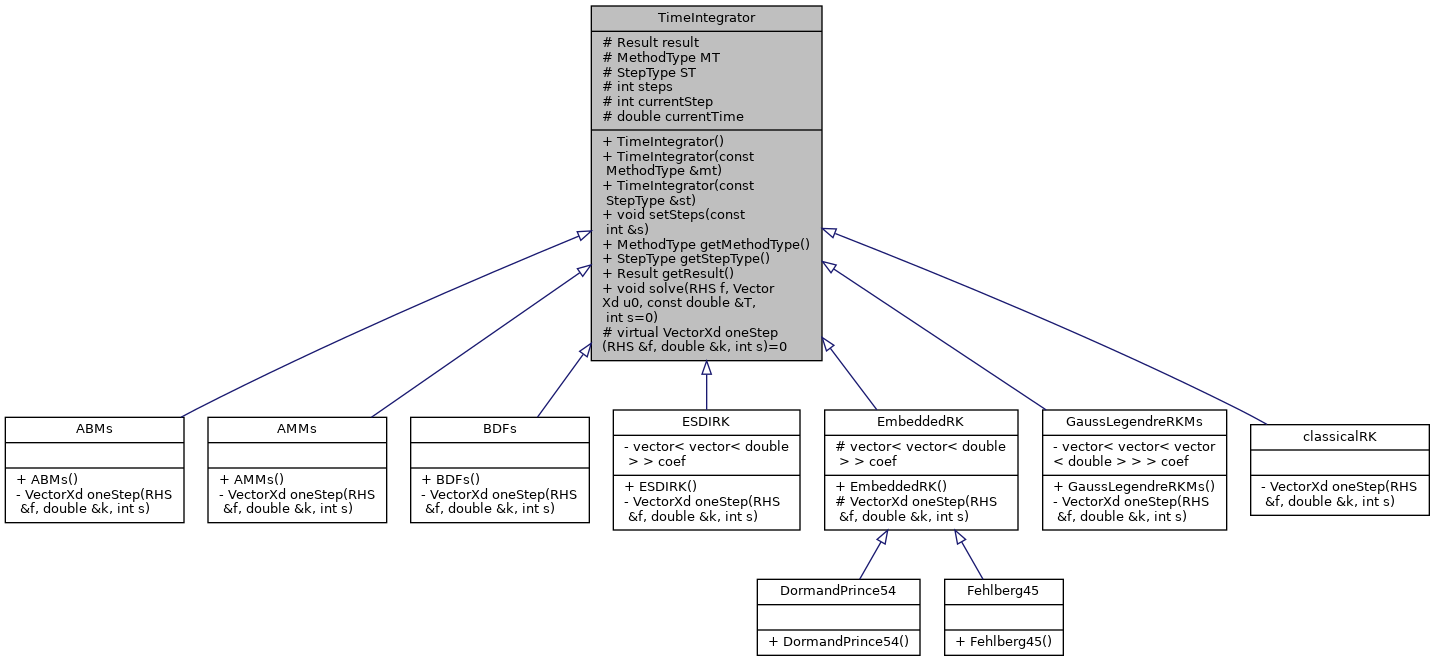
\includegraphics[width = \linewidth]{UML.png}
\end{figure}

\subsubsection{基类}

为了减少代码重复,提供了一个统一的求解接口给所有方法(单步/线性多步;固定步长/自适应步长)

参数$s$表示step(LMM)/stage(RK),当$s=0$缺省时代表其为不可选项
\begin{lstlisting}
void TimeIntegrator::solve( RHS f, VectorXd u0, const double & T, int s = 0 ){
    result.clear();
    currentStep = 0;
    currentTime = 0;
    result.U.push_back(u0);
    double k = T/steps;
    if( MT == LLM ){
        for( ; currentStep < s-1; currentStep++ ){
            VectorXd u(result.U.back());
            VectorXd y = f(u,currentStep*k);
            for( int i = 0; i < 4; i++ ){
                y = f(result.U.back()+k*CRKc[i]*y,currentStep*k+CRKc[i]*k);
                u = u + k*CRKb[i]*y;
            }
            result.U.push_back(u);
        }
    }
    if( ST == fixed ) for( ; (currentStep < steps) ; currentStep++ ) 
                            result.U.push_back( oneStep( f, k, s ) );
    else for( ; (currentTime < T) ; currentStep++ ) 
            result.U.push_back( oneStep( f, k, s ) );
    result.step = currentStep;
    result.time = currentTime;
}
\end{lstlisting}

通过派生类利用基类实现的构造函数来标识线性多步法/单步法,固定步长/自适应步长(默认为固定步长的单步法)
,并复写纯虚函数$oneStep(\cdots)$来实现对应的算法。
\begin{lstlisting}
    virtual TimeIntegrator::VectorXd oneStep( RHS & f, double & k, int s ) = 0;
\end{lstlisting}
这里传入的步长$k$为引用是为了适配自适应步长对k的更改。

\subsubsection{派生类(具体算法)}
为了对不同的LMM/RK根据其实际的系数表进行一些优化,不将其继承为LLM/RK,而是直接继承为具体算法,如(2.1.1)类图所示。

\paragraph{LMM 启动项} 由于对初始误差较敏感,若使用对应的低阶方法启动将会影响算法实际精度,在程序中统一用四阶经典RK方法启动,见2.1.2代码。

\paragraph{Butcher tableau of RK 的存储} 除四阶经典RK方法(用两个数组存储$\mathbf{c}$和$\mathbf{b}$即可)外其他方法均用二维动态数组\verb|vector<vector<double>>|存储,并将系数$\mathbf{b}$存至第一行(若需要)(Embedded RK 的$\mathbf{\hat{b}}$存在第二行),其余系数存储顺序同Butcher tableau相同。

\paragraph{非线性方程组求解} 除$Adams-Moulton\ methods$外其他方法均采用不动点迭代进行求解,而$Adams-Moulton\ methods$采用预估-校正的方法,即用显式的$Adams-Bashforth\ methods$先预估当前所需要的值再代入隐式的$Adams-Moulton\ methods$算法校正得到更精确的值。

\subsection{TimeIntegratorFactory}

基本照搬了助教所给的样例,这里就不再多赘述了

\subsection{UnitTest}

使用\verb|Catch2|单元测试框架,将测试分为Fixed Step Method、Adaptive Step Method、Compare Different Method三个Test Case,并在其内部分出SECTION并读取JSON文件来创建对应方法的SECTION实现了可以对每个方法进行独立的测试,并且增加或删除方法对应的SECTION只用在JSON文件中修改不用重新编译。

PS:测试中的断言只检测是否正常打开读取文件,以及工厂能否生成相对应的对象,不能检测算法精度是否达到要求。

\subsubsection{测试使用说明}

\begin{verbatim}
:./bin$ ./test -l # 列出所有的test case的名字和标签
All available test cases:
  Compare Different Method
      [TimeIntegrator]
  Adaptive Step Method
      [TimeIntegrator]
  Fixed Step Method
      [TimeIntegrator]
3 test cases
:./bin$ ./test testName # 运行对应名称的test case(名称中的空格需要加转义符号或用双引号括起来)
:./bin$ ./test [tag] # 运行所有包含该[tag]的test case 
:./bin$ ./test testName -c sectionName # 运行testName中sectionName 部分,-c 可以不断向下
:./bin$ ./test Fixed\ Step\ Method -c “(10.190)” -c "AMMs" -c 4
# 如上可以单独测试4阶精度Adams-Moulton方法
\end{verbatim}

\section{数值实验}

\subsection{概述}
\begin{itemize}
    \item 编写相应程序
    \item 求解如下 restricted three-body system 
    $$
    \left\{\begin{aligned}
        u_{1}^{\prime}= & u_{4} \\
        u_{2}^{\prime}= & u_{5}, \\
        u_{3}^{\prime}= & u_{6}, \\
        u_{4}^{\prime}= & 2 u_{5}+u_{1}-\frac{\mu\left(u_{1}+\mu-1\right)}{\left(u_{2}^{2}+u_{3}^{2}+\left(u_{1}+\mu-1\right)^{2}\right)^{3 / 2}} -\frac{(1-\mu)\left(u_{1}+\mu\right)}{\left(u_{2}^{2}+u_{3}^{2}+\left(u_{1}+\mu\right)^{2}\right)^{3 / 2}}, \\
        u_{5}^{\prime}= & -2 u_{4}+u_{2}-\frac{\mu u_{2}}{\left(u_{2}^{2}+u_{3}^{2}+\left(u_{1}+\mu-1\right)^{2}\right)^{3 / 2}}-\frac{(1-\mu) u_{2}}{\left(u_{2}^{2}+u_{3}^{2}+\left(u_{1}+\mu\right)^{2}\right)^{3 / 2}}, \\
        u_{6}^{\prime}= & -\frac{\mu u_{3}}{\left(u_{2}^{2}+u_{3}^{2}+\left(u_{1}+\mu-1\right)^{2}\right)^{3 / 2}} -\frac{(1-\mu) u_{3}}{\left(u_{2}^{2}+u_{3}^{2}+\left(u_{1}+\mu\right)^{2}\right)^{3 / 2}} .
        \end{aligned}\right.
    $$
    取$\mu = 0.012277471$,初值
    \begin{itemize}
        \item \textbf{(10.190):} $\mathbf{u}(0)=(0.994,0,0,0,-2.0015851063790825224,0),\ T_1 = 17.06521656015796$
        \item \textbf{(10.191):} $\mathbf{u}(0)=(0.879779227778,0,0,0,-0.379677780949,0),\ T_2 = 19.140540691377$
    \end{itemize}
    \item \textbf{判断与样例图像没有肉眼差别:} 当误差小于某个值同时步长小于某个值的时,步长太大即使误差很小也会使图像呈折线状 (比如自适应步长方法以及高阶精度的方法求解(10.191)
    \item \textbf{固定步长方法收敛阶判断:} 由于自适应步长方法步长并不固定,所以只测试验证固定步长方法的精度
    \begin{itemize}
        \item 对于(10.190)其误差由数值解与真解的差的绝对值所得到
        \item 对于(10.191)其误差由数值解与外推法所得到更精确的解的差的绝对值所得到,计算方式如下:
        
        设$U(k),U(\frac{k}{2})$分别是步长为$k,\ \frac{k}{2}$时的数值解
        
        $\hat{U} = U({\frac{k}{2}})+\frac{U({\frac{k}{2}})-U(k)}{2^p-1}$
        为计算$U(k)$的误差时所需要的更精确的解
    \end{itemize}
    对误差取最大模范数,并绘制$\log \|E\|_{\infty}$与步数取对数的关系图观察斜率判断收敛阶
    
    由于低阶精度方法收敛速度太慢的问题,这里对于(10.190)只测试3阶精度以上的方法,对于(10.191)只测试2阶精度以上的方法
    \item \textbf{自适应步长误差影响因素测试:}自适应步长的误差由每一步能够容忍的最大误差$\epsilon_i:=E_{abs,i}+|U_i^n|E_{rel,i}$控制,测试了$E_{abs},E_{rel}=\{10^{-3},1E0^{-8},10^{-13}\}$九种组合下的效果,测试初值使用(10.190)
    \item 比较初值(10.190)下24000步的Euler方法(一步ABM)、6000经典四阶RK、100步自适应步长Dormand-Prince5(4)嵌入式RK
    \item 对于初值(10.190)测试达到$10^{-3}$的误差哪种方法的耗时最短
\end{itemize}

\subsection{数值结果}

\subsubsection{固定步长方法}
下面将展示达到与样例无视觉差别的最大步长,以及误差下降曲线(蓝线)和耗时变化曲线(红线)
\paragraph{Adams-Bashforth methods}

\begin{enumerate}
    \item \textbf{s=2,p=2:}
    \begin{itemize}
        \item \textbf{(10.191)} \verb|Num of Step: 8000, max step length: 0.00239257|
        \begin{figure}[h]
            \centering
            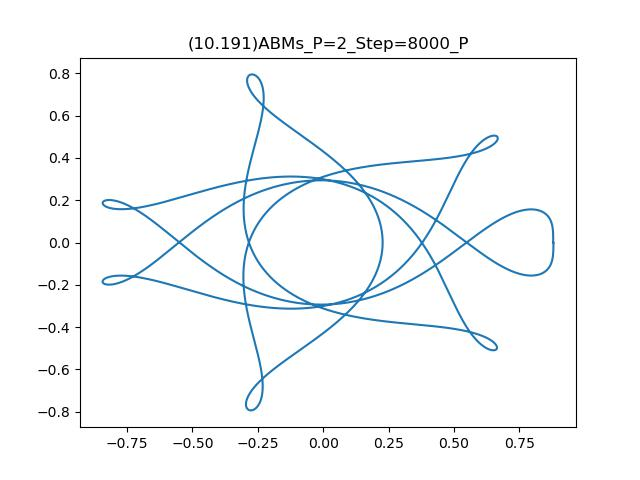
\includegraphics[width = 0.42\linewidth]{(10.191)ABMs_P=2_Step=8000_P.jpg}
            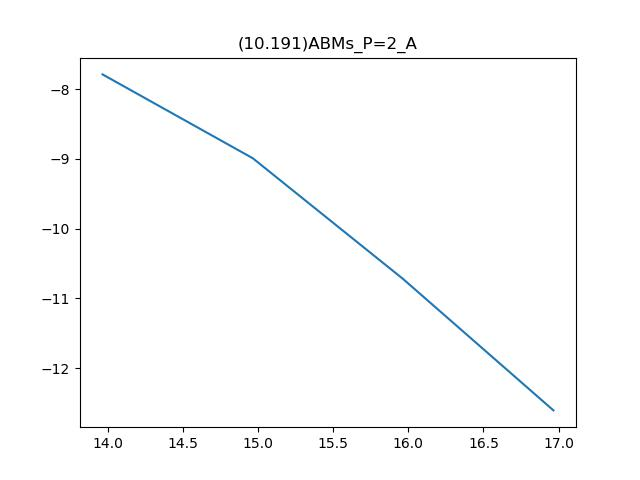
\includegraphics[width = 0.42\linewidth]{(10.191)ABMs_P=2_A.jpg}
        \end{figure}
    \end{itemize}
    \item \textbf{s=3,p=3:}
    \begin{itemize}
        \item \textbf{(10.190)} \verb|Num of Step: 48000, max step length: 0.000355525|
        \begin{figure}[h]
            \centering
            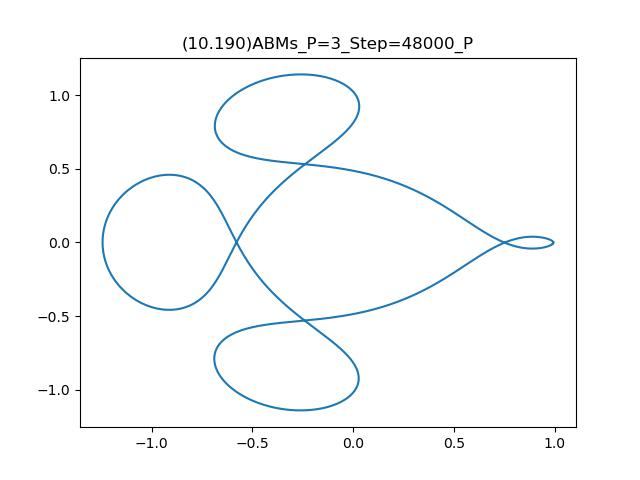
\includegraphics[width = 0.42\linewidth]{(10.190)ABMs_P=3_Step=48000_P.jpg}
            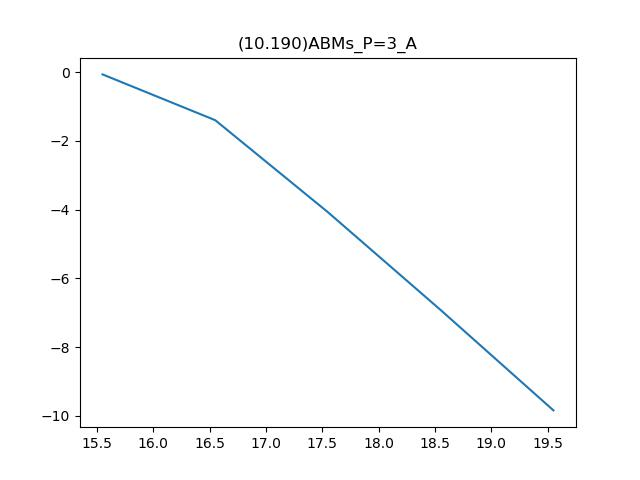
\includegraphics[width = 0.42\linewidth]{(10.190)ABMs_P=3_A.jpg}
        \end{figure}
        \item \textbf{(10.191)} \verb|Num of Step: 8000, max step length: 0.00239257|
        \begin{figure}[h]
            \centering
            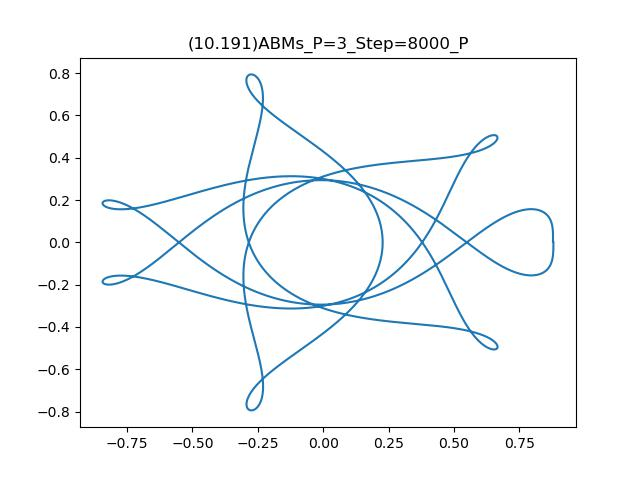
\includegraphics[width = 0.42\linewidth]{(10.191)ABMs_P=3_Step=8000_P.jpg}
            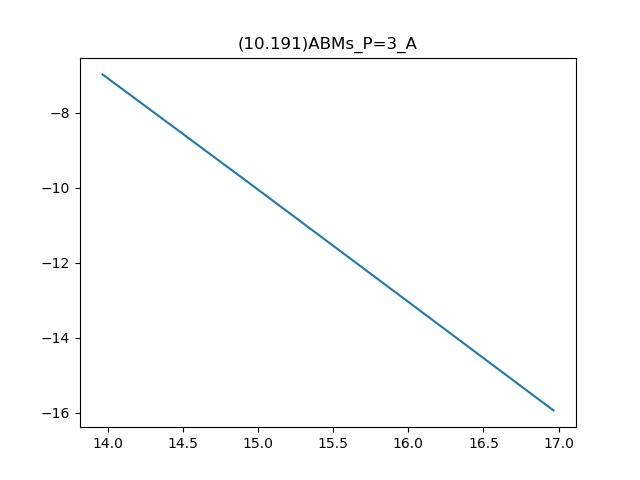
\includegraphics[width = 0.42\linewidth]{(10.191)ABMs_P=3_A.jpg}
        \end{figure}
    \end{itemize}
    \item \textbf{s=4,p=4:}
    \begin{itemize}
        \item \textbf{(10.190)} \verb|Num of Step: 96000, max step length: 0.000177763|
        \begin{figure}[h]
            \centering
            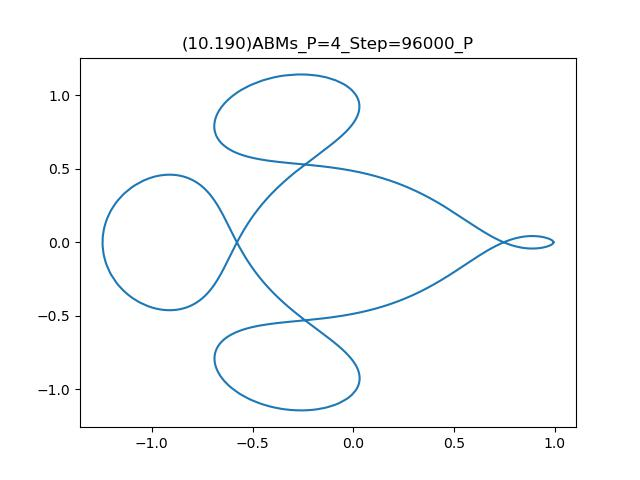
\includegraphics[width = 0.45\linewidth]{(10.190)ABMs_P=4_Step=96000_P.jpg}
            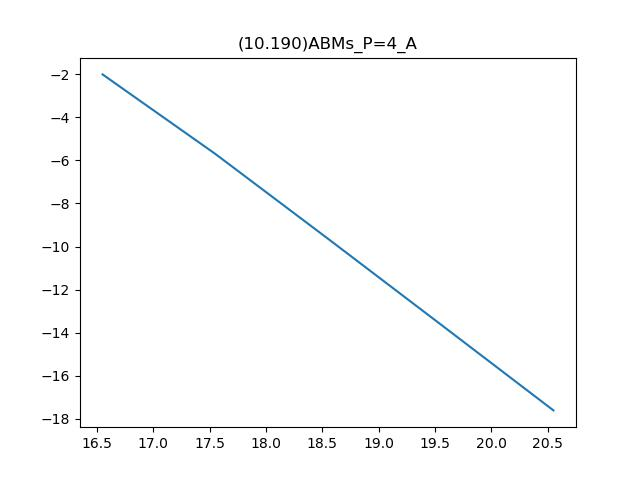
\includegraphics[width = 0.45\linewidth]{(10.190)ABMs_P=4_A.jpg}
        \end{figure}
        \item \textbf{(10.191)} \verb|Num of Step: 4000, max step length: 0.00478514|
        \begin{figure}[h]
            \centering
            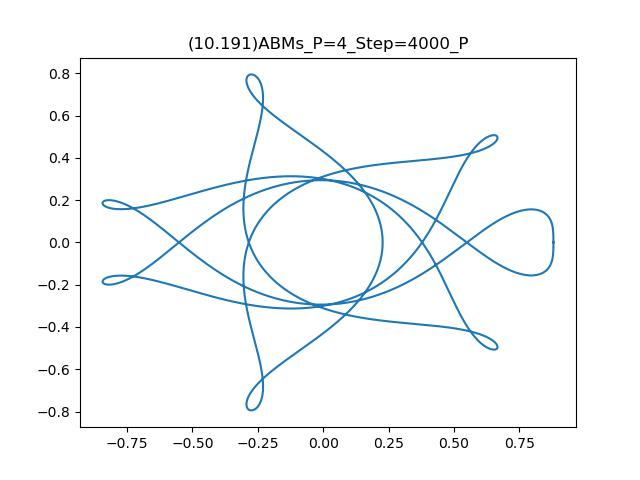
\includegraphics[width = 0.45\linewidth]{(10.191)ABMs_P=4_Step=4000_P.jpg}
            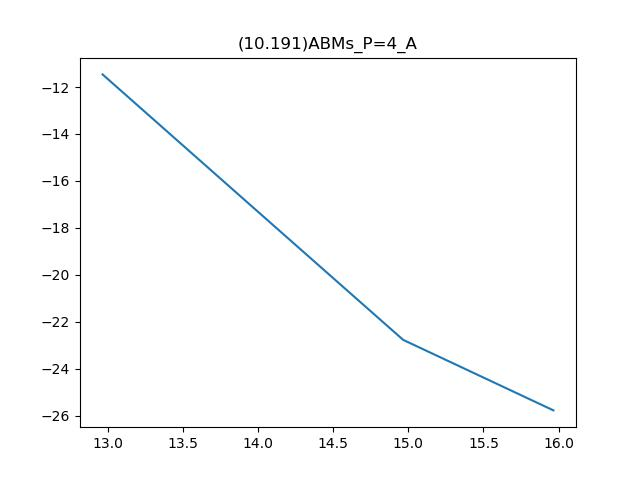
\includegraphics[width = 0.45\linewidth]{(10.191)ABMs_P=4_A.jpg}
        \end{figure}
    \end{itemize}
\end{enumerate}

\paragraph{Adams-Moulton methods}

\begin{enumerate}
    \item \textbf{s=1,p=2:}
    \begin{itemize}
        \item \textbf{(10.191)} \verb|Num of Step: 4000, max step length: 0.00478514|
        \begin{figure}[h]
            \centering
            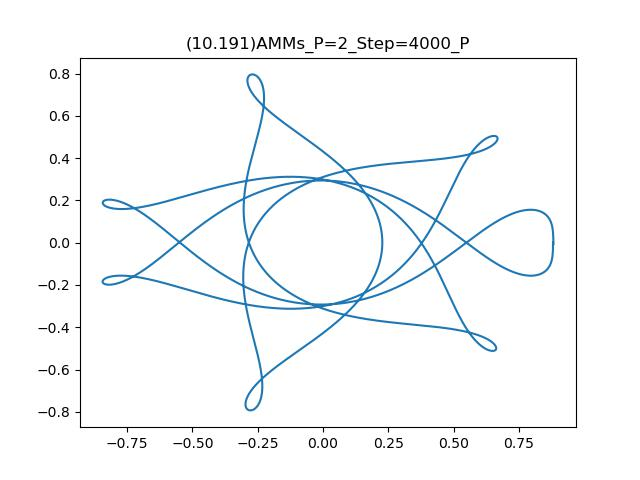
\includegraphics[width = 0.45\linewidth]{(10.191)AMMs_P=2_Step=4000_P.jpg}
            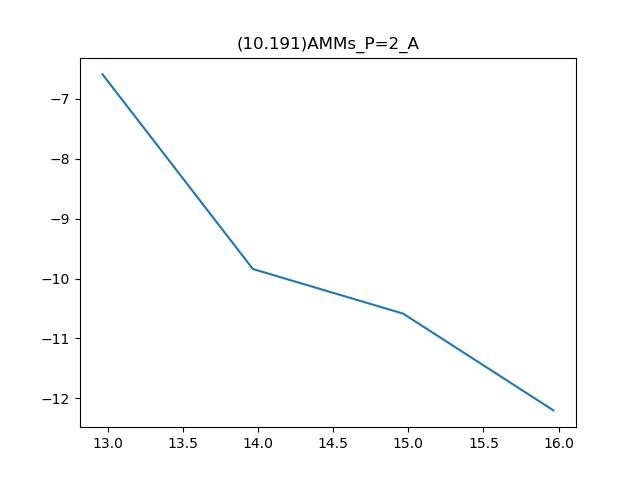
\includegraphics[width = 0.45\linewidth]{(10.191)AMMs_P=2_A.jpg}
        \end{figure}
    \end{itemize}
    \newpage
    \item \textbf{s=2,p=3:}
    \begin{itemize}
        \item \textbf{(10.190)} \verb|Num of Step: 96000, max step length: 0.000177763|
        \begin{figure}[h]
            \centering
            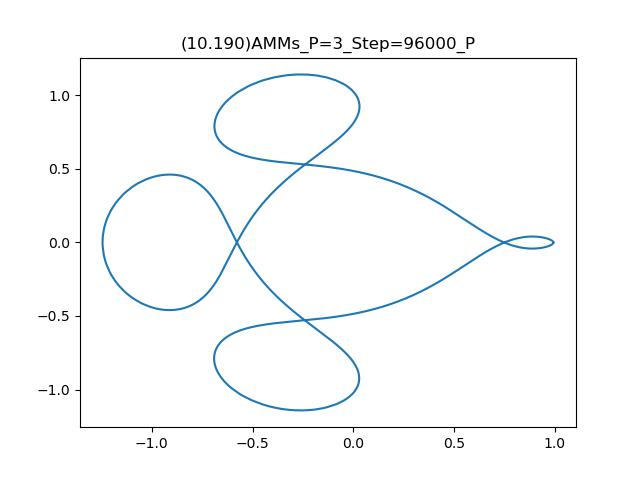
\includegraphics[width = 0.45\linewidth]{(10.190)AMMs_P=3_Step=96000_P.jpg}
            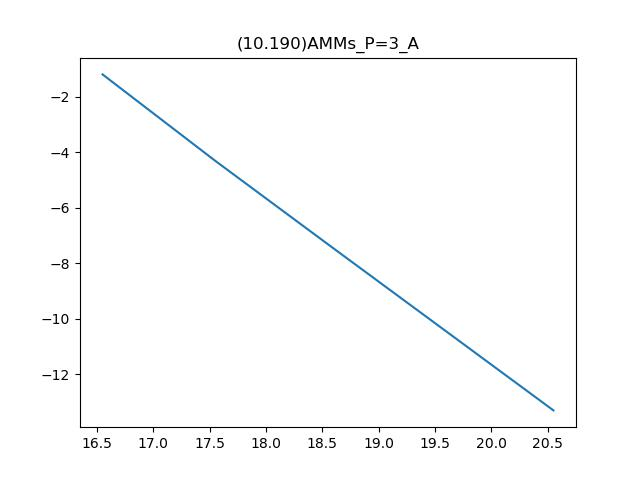
\includegraphics[width = 0.45\linewidth]{(10.190)AMMs_P=3_A.jpg}
        \end{figure}
        \item \textbf{(10.191)} \verb|Num of Step: 8000, max step length: 0.00239257|
        \begin{figure}[h]
            \centering
            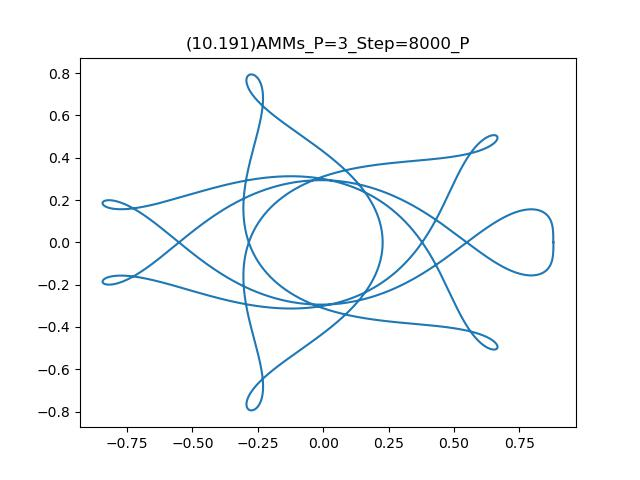
\includegraphics[width = 0.45\linewidth]{(10.191)AMMs_P=3_Step=8000_P.jpg}
            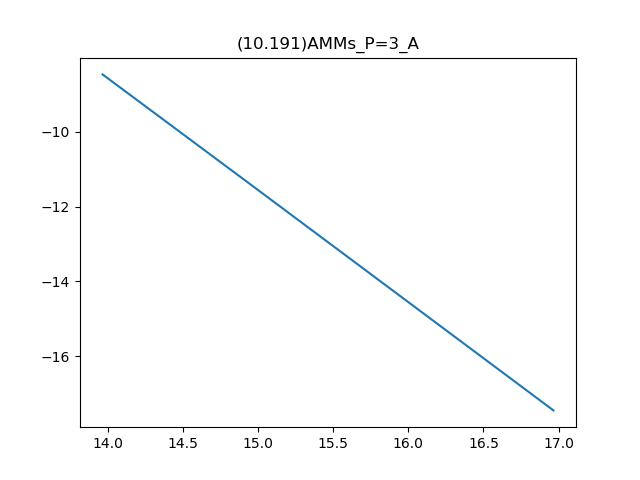
\includegraphics[width = 0.45\linewidth]{(10.191)AMMs_P=3_A.jpg}
        \end{figure}
    \end{itemize}
    \item \textbf{s=3,p=4:}
    \begin{itemize}
        \item \textbf{(10.190)} \verb|Num of Step: 48000, max step length: 0.000355525|
        \begin{figure}[h]
            \centering
            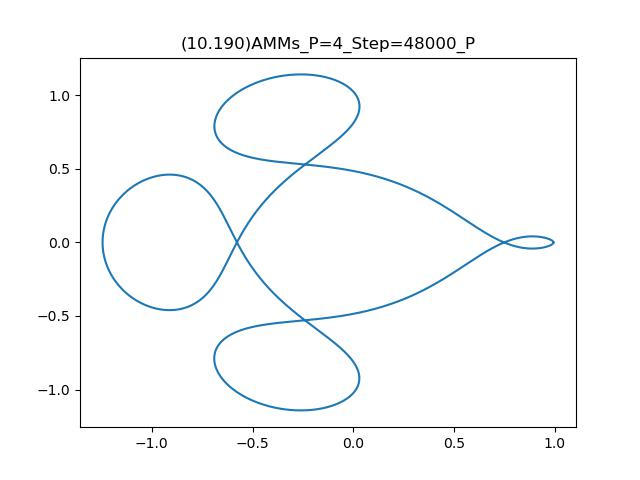
\includegraphics[width = 0.45\linewidth]{(10.190)AMMs_P=4_Step=48000_P.jpg}
            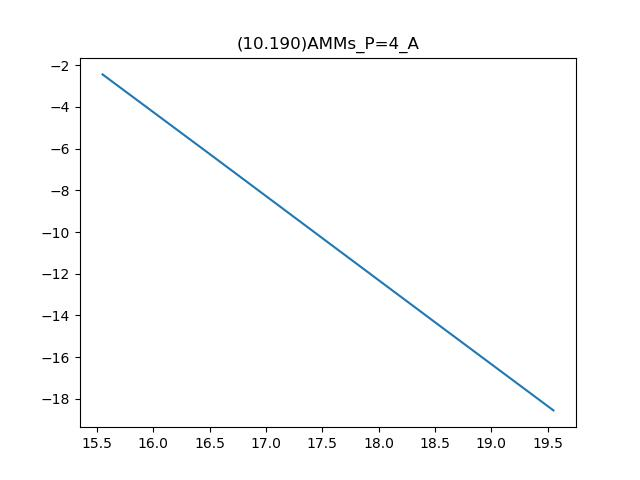
\includegraphics[width = 0.45\linewidth]{(10.190)AMMs_P=4_A.jpg}
        \end{figure}

        \newpage
        \item \textbf{(10.191)} \verb|Num of Step: 2000, max step length: 0.00957027|
        \begin{figure}[h]
            \centering
            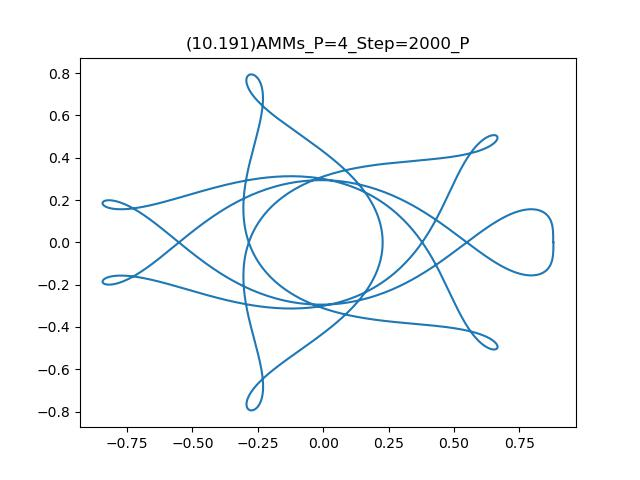
\includegraphics[width = 0.45\linewidth]{(10.191)AMMs_P=4_Step=2000_P.jpg}
            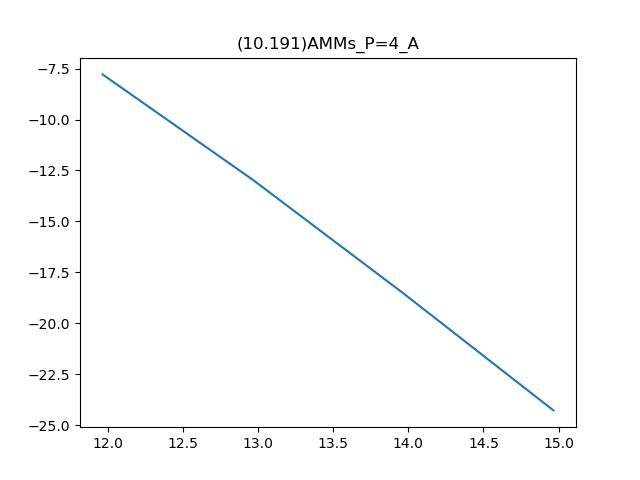
\includegraphics[width = 0.45\linewidth]{(10.191)AMMs_P=4_A.jpg}
        \end{figure}
    \end{itemize}
    \item \textbf{s=4,p=5:}
    \begin{itemize}
        \item \textbf{(10.190)} \verb|Num of Step: 24000, max step length: 0.000711051|
        \begin{figure}[h]
            \centering
            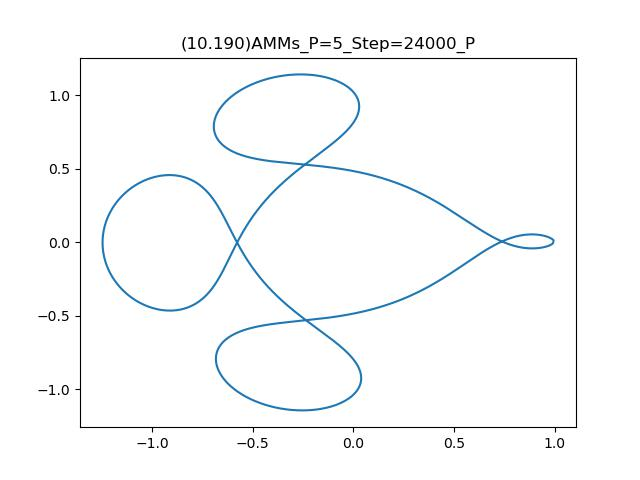
\includegraphics[width = 0.45\linewidth]{(10.190)AMMs_P=5_Step=24000_P.jpg}
            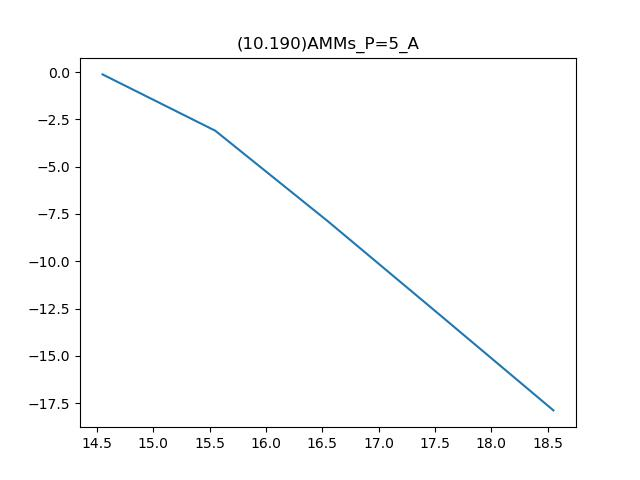
\includegraphics[width = 0.45\linewidth]{(10.190)AMMs_P=5_A.jpg}
        \end{figure}
        \item \textbf{(10.191)} \verb|Num of Step: 2000, max step length: 0.00957027|
        \begin{figure}[h]
            \centering
            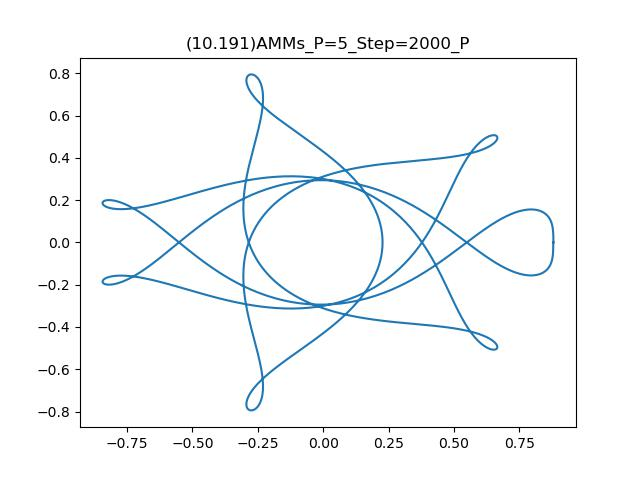
\includegraphics[width = 0.45\linewidth]{(10.191)AMMs_P=5_Step=2000_P.jpg}
            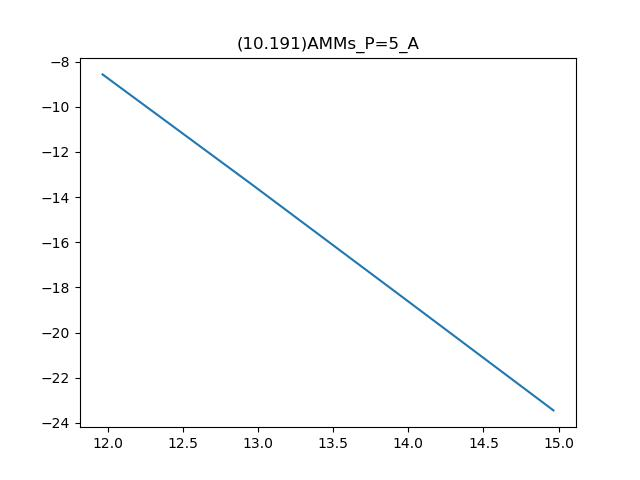
\includegraphics[width = 0.45\linewidth]{(10.191)AMMs_P=5_A.jpg}
        \end{figure}
    \end{itemize}
\end{enumerate}

\newpage

\paragraph{Backward differentiation formulas}

\begin{enumerate}
    \item \textbf{s=2,p=2:}
    \begin{itemize}
        \item \textbf{(10.191)} \verb|Num of Step: 8000, max step length: 0.00239257|
        \begin{figure}[h]
            \centering
            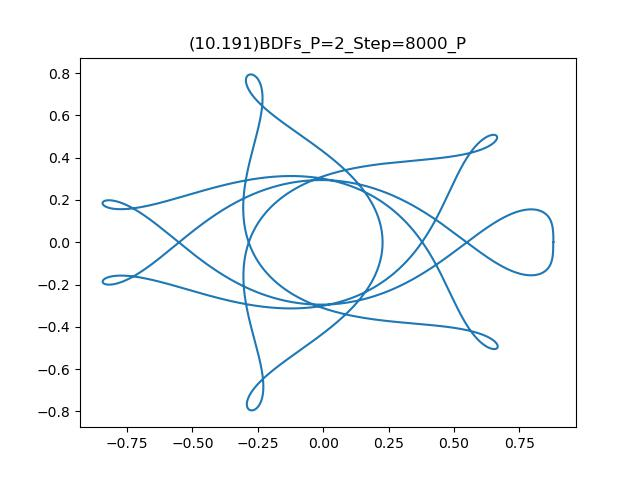
\includegraphics[width = 0.45\linewidth]{(10.191)BDFs_P=2_Step=8000_P.jpg}
            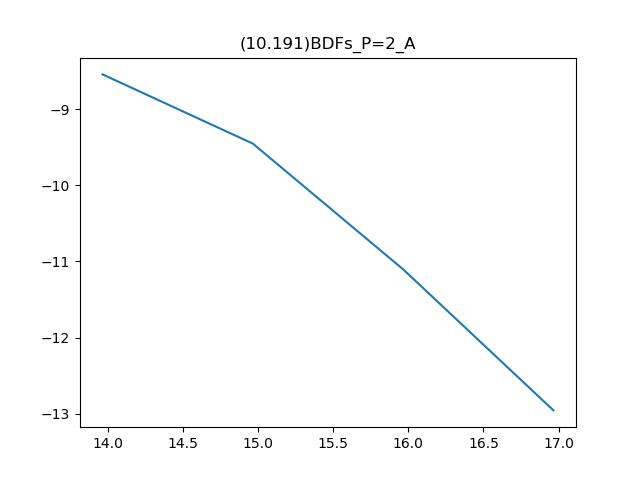
\includegraphics[width = 0.45\linewidth]{(10.191)BDFs_P=2_A.jpg}
        \end{figure}
    \end{itemize}
    \item \textbf{s=3,p=3:}
    \begin{itemize}
        \item \textbf{(10.190)} \verb|Num of Step: 48000, max step length: 0.000355525|
        \begin{figure}[h]
            \centering
            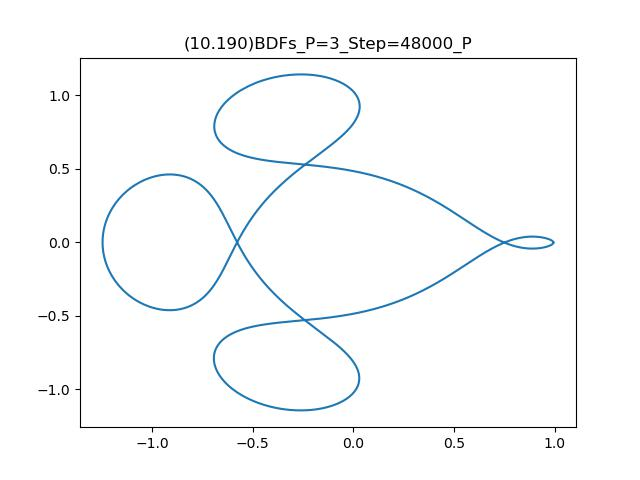
\includegraphics[width = 0.45\linewidth]{(10.190)BDFs_P=3_Step=48000_P.jpg}
            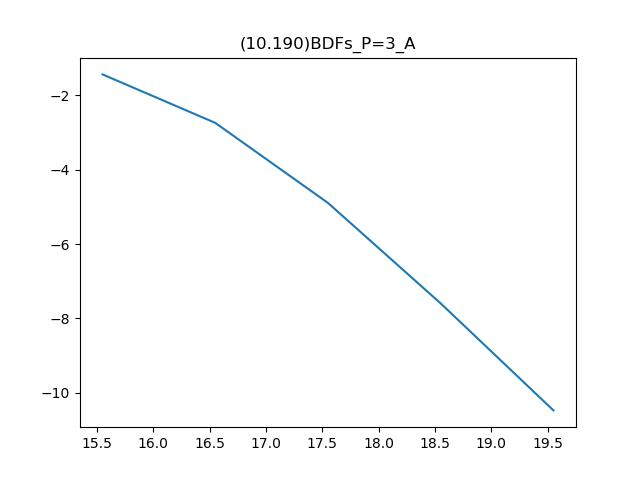
\includegraphics[width = 0.45\linewidth]{(10.190)BDFs_P=3_A.jpg}
        \end{figure}
        \item \textbf{(10.191)} \verb|Num of Step: 8000, max step length: 0.00239257|
        \begin{figure}[h]
            \centering
            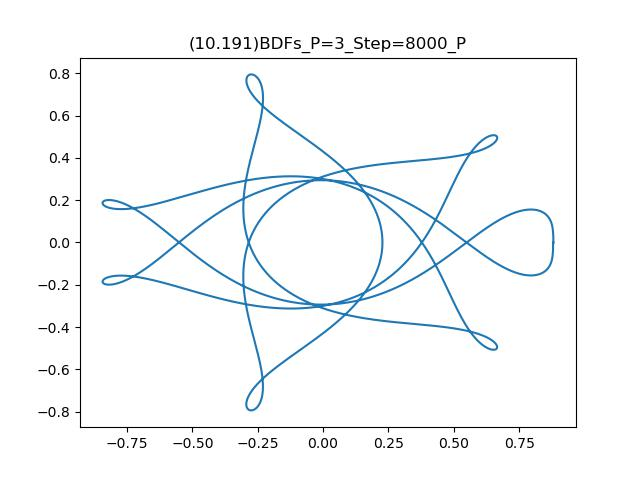
\includegraphics[width = 0.45\linewidth]{(10.191)BDFs_P=3_Step=8000_P.jpg}
            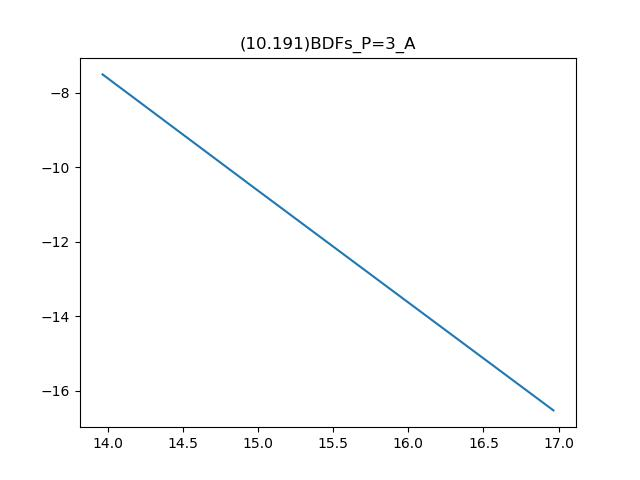
\includegraphics[width = 0.45\linewidth]{(10.191)BDFs_P=3_A.jpg}
        \end{figure}
    \end{itemize}
    \newpage
    \item \textbf{s=4,p=4:}
    \begin{itemize}
        \item \textbf{(10.190)} \verb|Num of Step: 96000, max step length: 0.000177763|
        \begin{figure}[h]
            \centering
            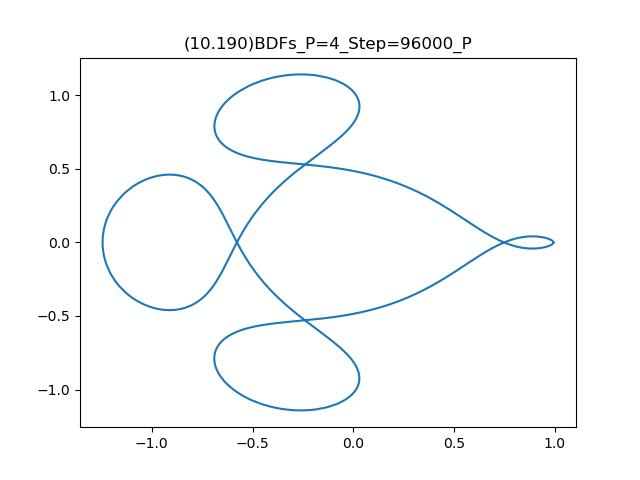
\includegraphics[width = 0.45\linewidth]{(10.190)BDFs_P=4_Step=96000_P.jpg}
            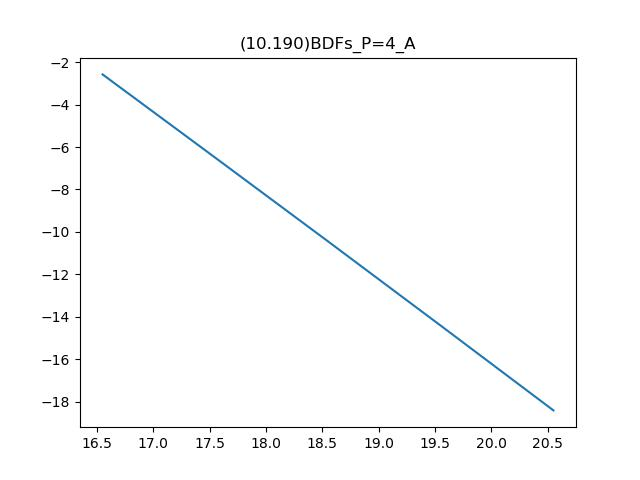
\includegraphics[width = 0.45\linewidth]{(10.190)BDFs_P=4_A.jpg}
        \end{figure}
        \item \textbf{(10.191)} \verb|Num of Step: 2000, max step length: 0.00957027|
        \begin{figure}[h]
            \centering
            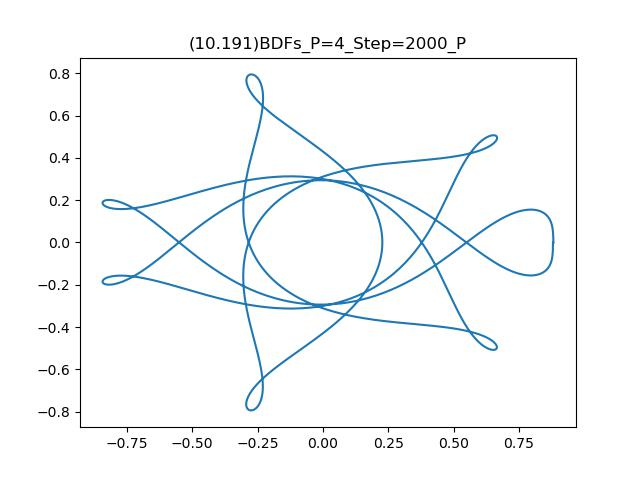
\includegraphics[width = 0.45\linewidth]{(10.191)BDFs_P=4_Step=2000_P.jpg}
            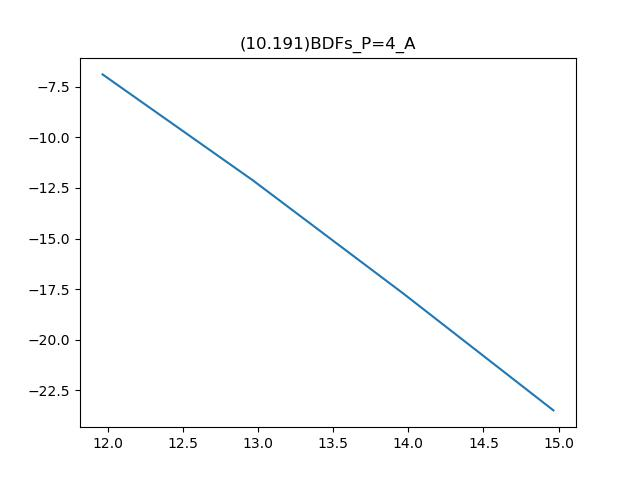
\includegraphics[width = 0.45\linewidth]{(10.191)BDFs_P=4_A.jpg}
        \end{figure}
    \end{itemize}
\end{enumerate}

\paragraph{Classicial RK method}

\begin{itemize}
    \item \textbf{(10.190)} \verb|Num of Step: 24000, max step length: 0.000711051|
    \begin{figure}[h]
        \centering
        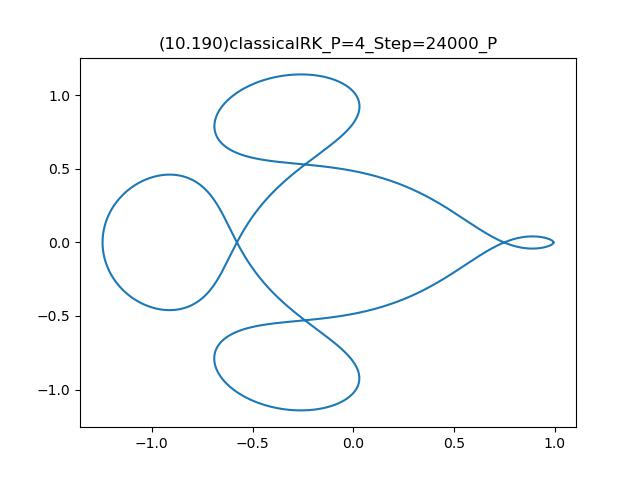
\includegraphics[width = 0.45\linewidth]{(10.190)classicalRK_P=4_Step=24000_P.jpg}
        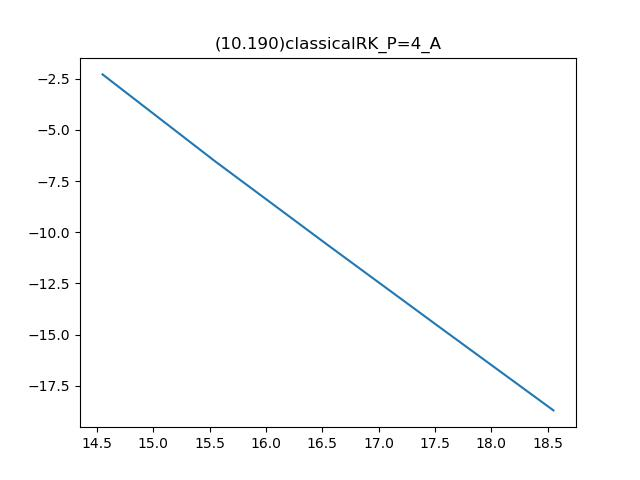
\includegraphics[width = 0.45\linewidth]{(10.190)classicalRK_P=4_A.jpg}
    \end{figure}
    \newpage
    \item \textbf{(10.191)} \verb|Num of Step: 1000, max step length: 0.0191405|
    \begin{figure}[h]
        \centering
        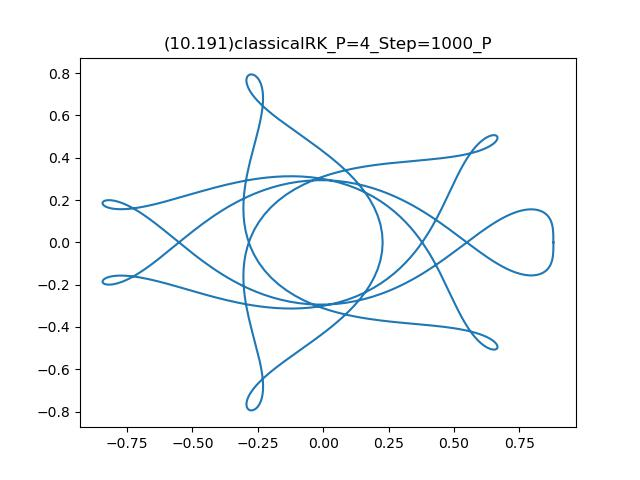
\includegraphics[width = 0.45\linewidth]{(10.191)classicalRK_P=4_Step=1000_P.jpg}
        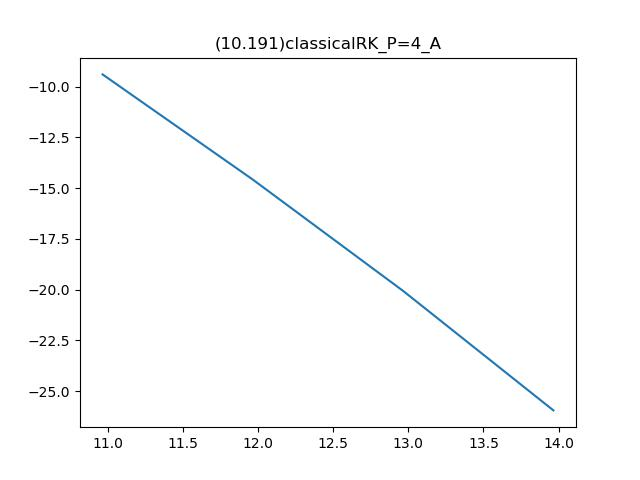
\includegraphics[width = 0.45\linewidth]{(10.191)classicalRK_P=4_A.jpg}
    \end{figure}
\end{itemize}

\paragraph{ESDIRK method}

\begin{itemize}
    \item \textbf{(10.190)} \verb|Num of Step: 24000, max step length: 0.000711051|
    \begin{figure}[h]
        \centering
        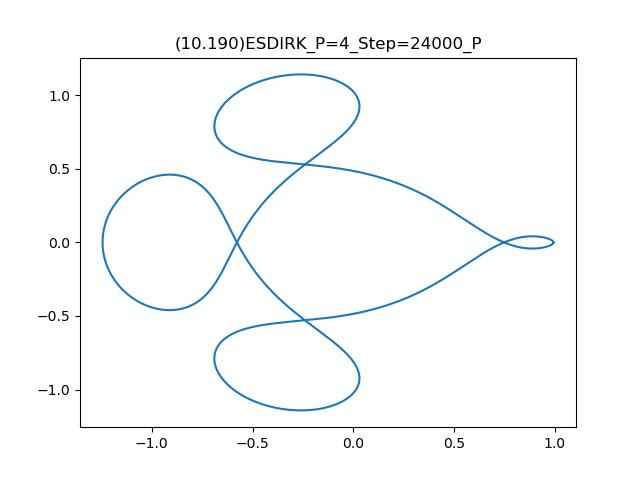
\includegraphics[width = 0.45\linewidth]{(10.190)ESDIRK_P=4_Step=24000_P.jpg}
        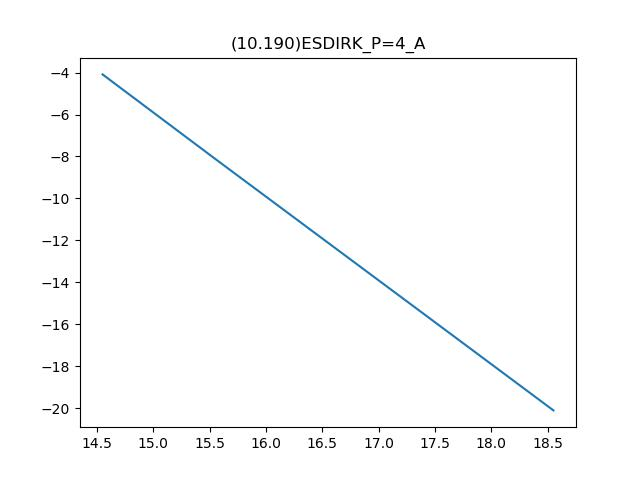
\includegraphics[width = 0.45\linewidth]{(10.190)ESDIRK_P=4_A.jpg}
    \end{figure}
    \item \textbf{(10.191)} \verb|Num of Step: 500, max step length: 0.0382811|
    \begin{figure}[h]
        \centering
        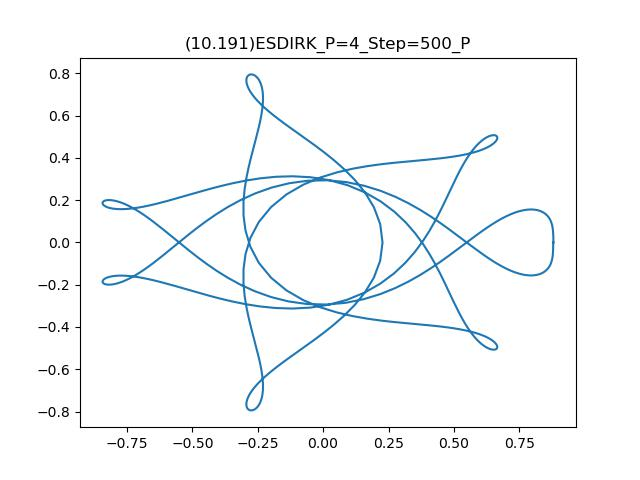
\includegraphics[width = 0.45\linewidth]{(10.191)ESDIRK_P=4_Step=500_P.jpg}
        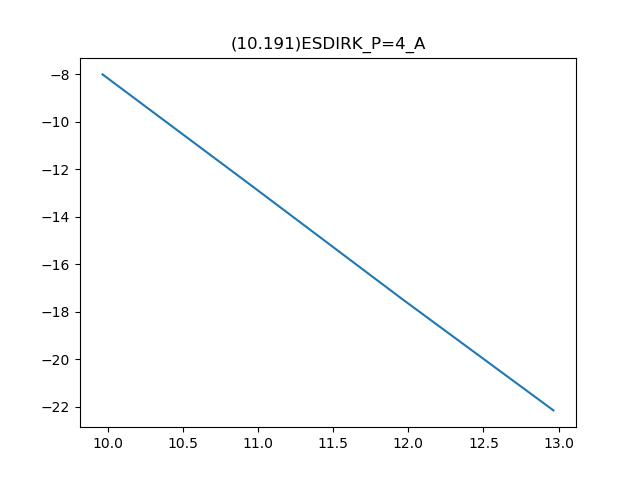
\includegraphics[width = 0.45\linewidth]{(10.191)ESDIRK_P=4_A.jpg}
    \end{figure}
\end{itemize}

\newpage

\paragraph{Gauss-Legendre RKMs}

\begin{enumerate}
    \item \textbf{s=1,p=2:}
    \begin{itemize}
        \item \textbf{(10.191)} \verb|Num of Step: 4000, max step length: 0.00478514|
        \begin{figure}[h]
            \centering
            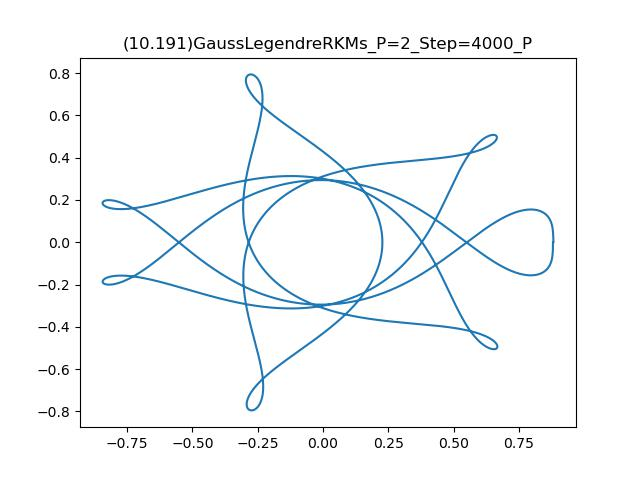
\includegraphics[width = 0.45\linewidth]{(10.191)GaussLegendreRKMs_P=2_Step=4000_P.jpg}
            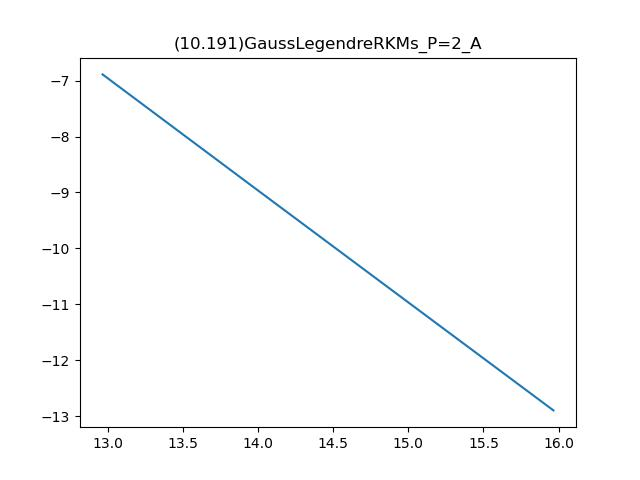
\includegraphics[width = 0.45\linewidth]{(10.191)GaussLegendreRKMs_P=2_A.jpg}
        \end{figure}
    \end{itemize}
    \item \textbf{s=2,p=4:}
    \begin{itemize}
        \item \textbf{(10.190)} \verb|Num of Step: 12000, max step length: 0.0014221|
        \begin{figure}[h]
            \centering
            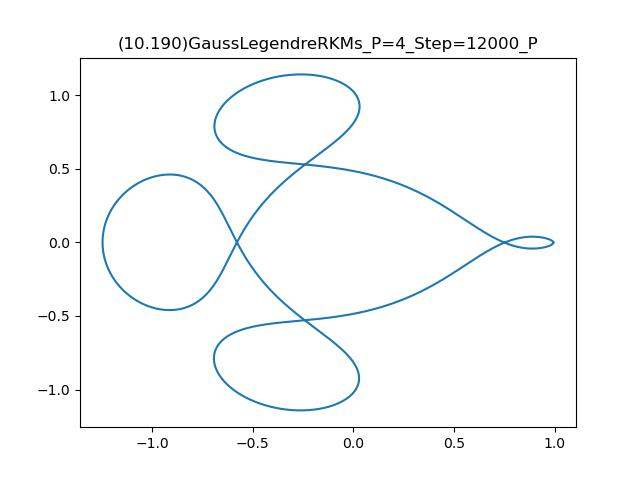
\includegraphics[width = 0.45\linewidth]{(10.190)GaussLegendreRKMs_P=4_Step=12000_P.jpg}
            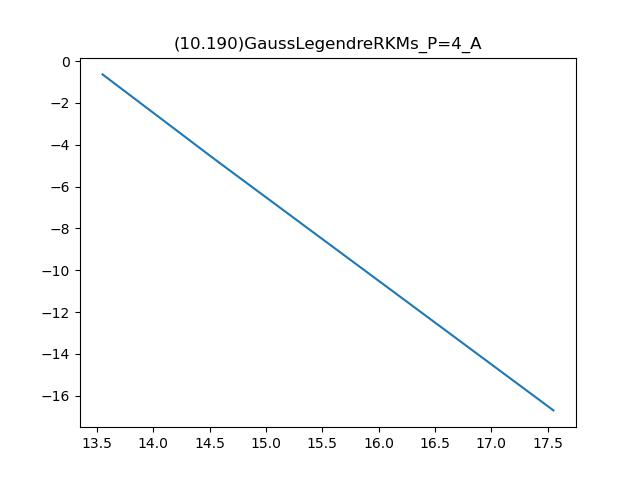
\includegraphics[width = 0.45\linewidth]{(10.190)GaussLegendreRKMs_P=4_A.jpg}
        \end{figure}
        \item \textbf{(10.191)} \verb|Num of Step: 500, max step length: 0.0382811|
        \begin{figure}[h]
            \centering
            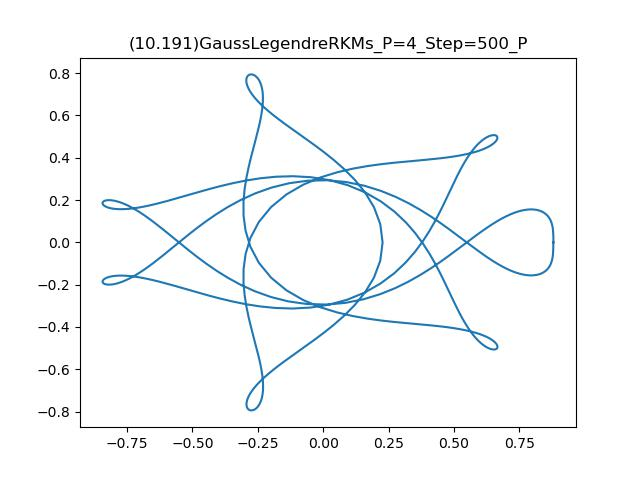
\includegraphics[width = 0.45\linewidth]{(10.191)GaussLegendreRKMs_P=4_Step=500_P.jpg}
            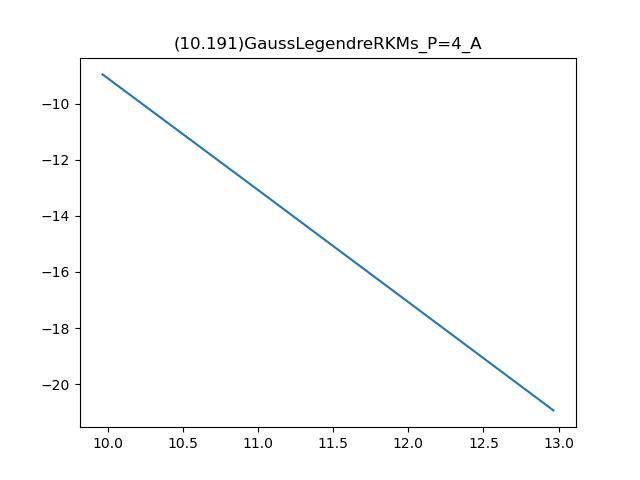
\includegraphics[width = 0.45\linewidth]{(10.191)GaussLegendreRKMs_P=4_A.jpg}
        \end{figure}
    \end{itemize}
    \newpage
    \item \textbf{s=3,p=6:}
    \begin{itemize}
        \item \textbf{(10.190)} \verb|Num of Step: 6000, max step length: 0.0028442|
        \begin{figure}[h]
            \centering
            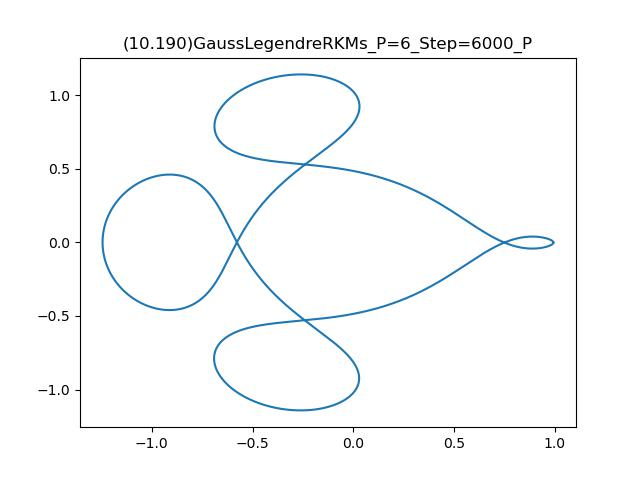
\includegraphics[width = 0.45\linewidth]{(10.190)GaussLegendreRKMs_P=6_Step=6000_P.jpg}
            \includegraphics[width = 0.45\linewidth]{(10.190)GaussLegendreRKMs_P=6_A.jpg}
        \end{figure}
        \item \textbf{(10.191)} \verb|Num of Step: 500, max step length: 0.0382811|
        \begin{figure}[h]
            \centering
            \includegraphics[width = 0.45\linewidth]{(10.191)GaussLegendreRKMs_P=6_Step=500_P.jpg}
            \includegraphics[width = 0.45\linewidth]{(10.191)GaussLegendreRKMs_P=6_A.jpg}
        \end{figure}
    \end{itemize}

    \item \textbf{s=4,p=8:}
    \begin{itemize}
        \item \textbf{(10.190)} \verb|Num of Step: 6000, max step length: 0.0028442|
        \begin{figure}[h]
            \centering
            \includegraphics[width = 0.45\linewidth]{(10.190)GaussLegendreRKMs_P=8_Step=6000_P.jpg}
            \includegraphics[width = 0.45\linewidth]{(10.190)GaussLegendreRKMs_P=8_A.jpg}
        \end{figure}
        \newpage
        \item \textbf{(10.191)} \verb|Num of Step: 500, max step length: 0.0382811|
        \begin{figure}[h]
            \centering
            \includegraphics[width = 0.45\linewidth]{(10.191)GaussLegendreRKMs_P=8_Step=500_P.jpg}
            \includegraphics[width = 0.45\linewidth]{(10.191)GaussLegendreRKMs_P=8_A.jpg}
        \end{figure}
    \end{itemize}

    \item \textbf{s=5,p=10:}
    \begin{itemize}
        \item \textbf{(10.190)} \verb|Num of Step: 3000, max step length: 0.00568841|
        \begin{figure}[h]
            \centering
            \includegraphics[width = 0.45\linewidth]{(10.190)GaussLegendreRKMs_P=10_Step=3000_P.jpg}
            \includegraphics[width = 0.45\linewidth]{(10.190)GaussLegendreRKMs_P=10_A.jpg}
        \end{figure}
        \item \textbf{(10.191)} \verb|Num of Step: 500, max step length: 0.0382811|
        \begin{figure}[h]
            \centering
            \includegraphics[width = 0.45\linewidth]{(10.191)GaussLegendreRKMs_P=10_Step=500_P.jpg}
            \includegraphics[width = 0.45\linewidth]{(10.191)GaussLegendreRKMs_P=10_A.jpg}
        \end{figure}
    \end{itemize}
    
\end{enumerate}

我们可以发现8阶和10阶精度方法的误差下降曲线最后一段呈水平状,这是因为已经触及到机器精度的界了

同时对于初值(10.191),6阶、8阶、10阶精度的方法分别在250步、125步、125步就达到了预设误差,只是步长太大可以看到明显的折线,如下图所示

\newpage

\begin{figure}[h]
    \centering
    \includegraphics[width = 0.32\linewidth]{(10.191)GaussLegendreRKMs_P=6_Step=250_P.jpg}
    \includegraphics[width = 0.32\linewidth]{(10.191)GaussLegendreRKMs_P=8_Step=125_P.jpg}
    \includegraphics[width = 0.32\linewidth]{(10.191)GaussLegendreRKMs_P=10_Step=125_P.jpg}
\end{figure}

\paragraph{小结} 从上面的图像可以看出所有的方法都符合理论的收敛精度,但是可以发现所有的四阶精度方法在求解初值(10.191)时会达到实际五阶的收敛精度,猜测是因为在该初值情况下其一步误差的$k^5$项系数始终为0;考虑到耗时较短时受CPU频率波动影响较大,从耗时曲线可以验证所有方法都是$O(\frac{1}{k})$的时间复杂度。

从达到预期视觉效果的角度看,最大步长一般来说随着精度的提高而减少,但是并不是绝对的,对于(10.190)ABMs和BDFs的四阶方法就需要比三阶方法更小的步长(不过也有可能是预设判断条件的影响)。并且同样是四阶方法,ABM、AMM、BDF、classical RK、ESDIRK、GLRK之间也有很大的差距。

\subsubsection{自适应步长方法}

由于自适应步长的效果受$E_{abs}$和$E_{rel}$控制,下边将展示达到无视觉差异所需要的误差限制,同时由于步长的变化,其迭代停止的条件是计算时间大于预设是时间,所以所得到的结果会有时域上的偏离,下面的$StopTime$即实际计算时对应的时间。

此外其实这两种自适应步长方法在100步左右就达到要求误差界,但是和高阶精度相同,步长太大导致有明显的折线出现(效果见3.2.3),所以加上了步数的要求以达到相应的视觉效果

\paragraph{Fehlberg 4(5) embedded RK method}

\begin{itemize}
    \item \textbf{(10.190)} \verb|Eabs: 1e-07, Erel: 1e-06, StopTime: 17.0654, step: 202|
    \begin{figure}[h]
        \centering
        \includegraphics[width = 0.7\linewidth]{(10.190)Fehlberg45_Step=202_P.jpg}
    \end{figure}
    \newpage
    \item \textbf{(10.191)} \verb|Eabs: 1e-07, Erel: 1e-06, StopTime: 19.1503, step: 313|
    \begin{figure}[h]
        \centering
        \includegraphics[width = 0.7\linewidth]{(10.191)Fehlberg45_Step=313_P.jpg}
    \end{figure}
\end{itemize}


\paragraph{Dormand-Prince 5(4) embedded RK method}

\begin{itemize}
    \item \textbf{(10.190)} \verb|Eabs: 1e-07, Erel: 1e-06, StopTime: 17.0654, step: 185|
    \begin{figure}[h]
        \centering
        \includegraphics[width = 0.7\linewidth]{(10.190)DormandPrince54_Step=185_P.jpg}
    \end{figure}
    \newpage
    \item \textbf{(10.191)} \verb|Eabs: 1e-07, Erel: 1e-06, StopTime: 19.1467, step: 292|
    \begin{figure}[h]
        \centering
        \includegraphics[width = 0.7\linewidth]{(10.191)DormandPrince54_Step=292_P.jpg}
    \end{figure}
\end{itemize}

\paragraph{$\mathbf{E_{abs},E_{rel}}$ 影响测试}

测试初值条件使用(10.190)
\begin{itemize}
    \item \textbf{Fehlberg 4(5) embedded RK method}
\begin{verbatim}
Eabs: 0.001, Erel: 0.001, StopTime: 17.3853, step: 41  , Error: 1.89377
Eabs: 0.001, Erel: 1e-08, StopTime: 17.2026, step: 44  , Error: 1.98484
Eabs: 0.001, Erel: 1e-13, StopTime: 17.2026, step: 44  , Error: 1.98487
Eabs: 1e-08, Erel: 0.001, StopTime: 17.0659, step: 73  , Error: 1.58515
Eabs: 1e-08, Erel: 1e-08, StopTime: 17.0654, step: 384 , Error: 0.052968
Eabs: 1e-08, Erel: 1e-13, StopTime: 17.0653, step: 413 , Error: 0.0308044
Eabs: 1e-13, Erel: 0.001, StopTime: 17.0656, step: 76  , Error: 2.20126
Eabs: 1e-13, Erel: 1e-08, StopTime: 17.0653, step: 564 , Error: 0.0214348
Eabs: 1e-13, Erel: 1e-13, StopTime: 17.0652, step: 3807, Error: 0.0068447
\end{verbatim}

\item \textbf{Dormand-Prince 5(4) embedded RK method}
\begin{verbatim}
Eabs: 0.001, Erel: 0.001, StopTime: 17.5487, step: 39  , Error: 1.7923
Eabs: 0.001, Erel: 1e-08, StopTime: 17.5673, step: 42  , Error: 1.73972
Eabs: 0.001, Erel: 1e-13, StopTime: 17.5673, step: 42  , Error: 1.73974
Eabs: 1e-08, Erel: 0.001, StopTime: 17.0713, step: 61  , Error: 0.952661
Eabs: 1e-08, Erel: 1e-08, StopTime: 17.0654, step: 355 , Error: 0.0485328
Eabs: 1e-08, Erel: 1e-13, StopTime: 17.0653, step: 382 , Error: 0.0198613
Eabs: 1e-13, Erel: 0.001, StopTime: 17.0783, step: 61  , Error: 1.26465
Eabs: 1e-13, Erel: 1e-08, StopTime: 17.0652, step: 517 , Error: 0.00635806
Eabs: 1e-13, Erel: 1e-13, StopTime: 17.0652, step: 3514, Error: 0.00259308
\end{verbatim}

\end{itemize}

从上面的结果可以看出其效果由$E_{abs},E_{rel}$两者中的较大值决定,同时可以发现随着误差的不断减小,实际计算时间也在不断的逼近预设时间。

\subsubsection{Euler、CRK4、Dormand-Prince5(4) 比较}
\begin{verbatim}
    ABMs(s=1)      : step = 24000, Max-norm Error = 1.8898
    classicalRK    : step = 6000 , Max-norm Error = 2.06085
    DormandPrince54: step = 99   , Max-norm Error = 0.391498
\end{verbatim}
    \begin{figure}[h]
    \centering
    \includegraphics[width = 0.32\linewidth]{ABMs(s=1)_Step=24000_P.jpg}
    \includegraphics[width = 0.32\linewidth]{classicalRK_Step=6000_P.jpg}
    \includegraphics[width = 0.32\linewidth]{DormandPrince54_Step=99_P.jpg}
\end{figure}

可以发现Euler方法24000步时效果非常糟糕(实际上需要一百万步上才能达到比较好的效果),而6000步CRK4虽然已经能看出解的形状但是仍有不小的误差,而自适应步长的Dormand-Prince5(4)嵌入式RK方法只用了一百步就达到了很好的效果。

\subsubsection{耗时性能测试}
由3.2.1的测试结果我们首先排除低阶精度的固定步长方法,所以在其中选择十阶精度的GLRK方法与两种自适应步长进行比较,结果如下:
\begin{verbatim}
 GaussLegendreRKMs(s=5): step = 5000, CPU Time =441.184ms, Max-norm Error = 0.000902643
 Fehlberg45            : step = 6366, CPU Time =103.099ms, Max-norm Error = 0.000565425
 DormandPrince54       : step = 4848, CPU Time =93.6715ms, Max-norm Error = 0.000885535    
\end{verbatim}

三种方法均在5000步左右就可以将最大模误差降到$10^{-3}$以下,但是由于两种自适应步长方法为显式方法而GLRK则需要求解非线性方程,所以在耗时上明显劣于自适应方法,虽然Fehlberg4(5)在耗时上稍稍多于Dormand-Prince5(4),但是测试的误差较小,因此我认为这两种自适应步长方法在以$10^{-3}$误差界的前提下耗时性能上相差无几。

同时从结果上可以发现虽然F45要比DP54多出1500步左右,但是在耗时上却差不多,这是由于F45计算中少了一个stage抵消了步数较多的劣势。

ps:这里的测试受CPU频率并不固定影响较大,可能会出现较大的波动,可以通过限制CPU最大频率同时设置在运行时马上达到最大频率解决。

并且在\verb|bin|目录下执行\verb|./test "Compare Different Method" -c "Compare Time Performance"|进行多次单元测试。

\end{document}